\chapter{TINJAUAN PUSTAKA}
\label{chap:tinjauanpustaka}

% Ubah bagian-bagian berikut dengan isi dari tinjauan pustaka

\section{Penelitian Terdahulu}
\label{sec:21}

\subsection{\emph{Classification of Diabetic Retinopathy Based on B-ResNet}}
\label{subsec:211}

Zhang dan rekan \parencite{zhang2022residual} pada penelitiannya menggunakan data set Eye-PACS, MESSIDOR-2, dan IDRiD untuk membangun data set DR dengan pembersihan, penguatan, dan normalisasi gambar. Selain itu, digunakan metode prapemrosesan gambar yang ditingkatkan untuk meningkatkan fitur gambar fundus. Model B-ResNet dibangun dengan menggabungkan keunggulan ekstraksi fitur ResNet50 dan fusi fitur BCNN. Selain itu, sebelum fusi fitur, gambar fitur yang diekstraksi oleh ResNet50 diproses oleh modul perhatian saluran. ResNet50 dipralatih pada data set ImageNet dan parameternya di-fine-tune melalui transfer learning.

Hasil penelitian menunjukkan bahwa model B-ResNet mencapai akurasi 71,11\% , ACA 0,714, Kappa 0,634, dan macro-F1 0,711. Hasil ini lebih tinggi daripada penelitian sebelumnya. Percobaan perbandingan membuktikan bahwa metode prapemrosesan gambar yang ditingkatkan meningkatkan akurasi, ACA, Kappa, dan nilai macro-F1 model.

\subsection{\emph{A Deep Learning Framework for Detection and Classification of Diabetic Retinopathy in FundusImages Using Residual Neural Networks}}
\label{subsec:212}

Abini dan rekan \parencite{10335079} melakukan studi menggunakan model ResNet, yang dilatih dengan dataset APTOS, untuk melakukan klasifikasi biner dan multikelas menggunakan jaringan saraf konvolusional dalam (deep convolutional neural network). Hasil eksperimen menunjukkan bahwa model dengan lapisan dalam seperti ResNet-50 dapat meningkatkan kinerja keseluruhan dataset. Ini mengindikasikan bahwa penggunaan model ResNet-50 dalam klasifikasi DR dapat menjadi lebih efisien dalam hal waktu, tenaga kerja, dan biaya dibandingkan dengan metode diagnostik manual.

\section{Teori/Konsep Dasar}
\label{sec:22}

\subsection{Retinopati Diabetik}
Retinopati diabetik adalah komplikasi dari diabetes melitus yang mempengaruhi mata. Secara klinis, retinopati diabetik didefinisikan sebagai adanya tanda-tanda mikrovaskular retina yang khas pada seseorang dengan diabetes mellitus. Kehilangan penglihatan berkembang dari gejala sisa dari makulopati (edema makula dan iskemia) dan neovaskularisasi retina (vitreous perdarahan dan ablasi retina) dan iris (glaukoma neovaskular) \parencite{Cheung2010}. 
Hal ini disebabkan karena kerusakan pembuluh darah di retina, lapisan jaringan yang peka cahaya di belakang mata. Retinopati diabetik merupakan penyebab utama kebutaan pada populasi usia kerja di banyak negara \parencite{fong2004diabetic}.

Kondisi ini pertama kali diamati oleh Eduard Jaeger pada tahun 1856 pada Jurnalnya berjudul “Beitrage zur Pathologie des Auges” \parencite{jaeger1855}. Data lebih lanjut yang terdokumentasi dengan baik yang membuktikan hubungan sebab akibat antara diabetes dan makulopati baru muncul pada tahun 1869, ketika Henry Noyes menerbitkan laporannya di Amerika Serikat yang berjudul "Retinitis in Glycosuria." Pengamatan Noyes dikonfirmasi beberapa tahun kemudian, pada tahun 1872, oleh Edward Nettleship di London, yang mengembangkan lebih lanjut topik ini dalam makalahnya yang berjudul "On Edema or Cystic Diseases of the Retina." \parencite{Wolfensberger2001}.
%Penamaan Retinopati diabetik sendiri baru pertama kali digunakan pada 1906, oleh 

\subsubsection{Klasifikasi Retinopati Diabetik}

Retinopati diabetik dapat diklasifikasikan menjadi dua tahap utama:

\begin{enumerate}
    \item \textbf{Retinopati Diabetik Non-Proliferatif (RDN):} Pada tahap ini, dinding pembuluh darah di retina melemah. Mikroaneurisma dapat terjadi, yang menyebabkan kebocoran cairan dan darah ke dalam retina. Ini dapat mengakibatkan pembengkakan makula (edema makula) dan kehilangan penglihatan \parencite{aiello1998diabetic}.
    \item \textbf{Retinopati Diabetik Proliferatif (RDP):} Merupakan tahap lanjut dari retinopati diabetik. Pada RDP, pembuluh darah baru yang abnormal mulai tumbuh di retina. Pembuluh darah baru ini rapuh dan dapat berdarah ke dalam vitreous, menyebabkan penurunan penglihatan yang signifikan atau bahkan kebutaan \parencite{king1998diabetes}.
\end{enumerate}

\subsubsection{Faktor Risiko dan Patogenesis}

Beberapa faktor risiko untuk retinopati diabetik termasuk durasi diabetes, kontrol glukosa darah yang buruk, hipertensi, hiperlipidemia, dan kehamilan \parencite{fong2004diabetic}. Patogenesis retinopati diabetik melibatkan proses kompleks yang termasuk peningkatan permeabilitas vaskular, kerusakan kapiler, dan hipoksia retina, yang mendorong angiogenesis patologis \parencite{antonetti2012diabetic}.

\subsubsection{Diagnosis dan Pengobatan}

\begin{itemize}
    \item \textbf{Diagnosis:} Retinopati diabetik biasanya didiagnosis melalui pemeriksaan fundus menggunakan ophthalmoscopy atau fotografi fundus. Fluorescein angiography dan Optical Coherence Tomography (OCT) juga digunakan untuk mengevaluasi tingkat kerusakan retina \parencite{browning2008optical}.
    \item \textbf{Pengobatan:} Pengobatan retinopati diabetik mencakup kontrol ketat terhadap kadar gula darah, tekanan darah, dan kadar lipid. Terapi laser (panretinal photocoagulation) digunakan untuk mengatasi RDP dan edema makula. Injeksi intravitreal dari agen anti-VEGF (vascular endothelial growth factor) juga efektif dalam mengurangi edema makula dan mencegah pertumbuhan pembuluh darah baru yang abnormal \parencite{ciulla2003intravitreal}.
\end{itemize}

\subsection{Pengolahan Citra}
\label{sec:221}

Pengolahan citra adalah suatu proses yang mengubah citra menjadi citra lain yang lebih baik dan lebih sesuai dengan kebutuhan. Pengolahan citra dibagi menjadi dua, yaitu pengolahan citra analog dan pengolahan citra digital. Pengolahan citra analog adalah pengolahan citra yang dilakukan pada citra analog. Pengolahan citra digital adalah pengolahan citra yang dilakukan pada citra digital. Pengolahan citra digital dilakukan dengan menggunakan komputer. Pengolahan citra digital dibagi menjadi beberapa tahap, yaitu prapemrosesan, segmentasi, ekstraksi fitur, dan klasifikasi.

\subsection{OCT Angiography}
\label{sec:222}

OCT Angiography (OCTA) adalah teknologi pencitraan medis non-invasif yang memanfaatkan prinsip Optical Coherence Tomography (OCT) untuk memvisualisasi aliran darah mikro di retina dan koroid. OCTA memberikan informasi struktural dan fungsional jaringan mata secara simultan, memungkinkan diagnosis dan pemantauan penyakit mata yang lebih komprehensif \parencite{Kashani2017-hn}.

OCTA menggunakan deteksi perubahan temporal dalam reflektivitas untuk membedakan pembuluh darah dari jaringan statis, memungkinkan visualisasi struktur vaskular tanpa memerlukan pewarna kontras seperti fluorescein atau indocyanine green \parencite{jia2012split}.

\subsubsection{Prinsip Kerja}

OCTA bekerja dengan memanfaatkan teknologi Optical Coherence Tomography (OCT), yang menggunakan cahaya koheren untuk menghasilkan gambar resolusi tinggi dari struktur internal mata. Perbedaan utama antara OCT konvensional dan OCTA adalah kemampuan OCTA untuk mendeteksi pergerakan darah dalam pembuluh darah, sehingga memungkinkan pencitraan dinamis dari aliran darah \parencite{spaide2018choriocapillaris}.

\subsubsection{Aplikasi Klinis}

OCTA telah menjadi alat penting dalam diagnosis dan pemantauan berbagai penyakit mata, termasuk degenerasi makula terkait usia (AMD), retinopati diabetik, dan oklusi vena retina. OCTA memungkinkan visualisasi mikroaneurisma, iskemia kapiler, dan neovaskularisasi dengan detail yang tinggi, yang membantu dalam penilaian dan pengelolaan kondisi ini \parencite{de2016optical}.

\subsubsection{Keunggulan dan Keterbatasan}

\begin{itemize}
    \item \textbf{Keunggulan:} Keuntungan utama dari OCTA adalah non-invasif dan tidak memerlukan pewarna kontras, mengurangi risiko reaksi alergi dan komplikasi lainnya. Selain itu, OCTA menyediakan gambar resolusi tinggi dari lapisan vaskular yang berbeda dalam retina \parencite{spaide2018retinal}.
    \item \textbf{Keterbatasan:} Meskipun memiliki banyak keunggulan, OCTA juga memiliki keterbatasan. Salah satunya adalah sensitivitas terhadap gerakan pasien, yang dapat menghasilkan artefak dalam gambar. Selain itu, interpretasi gambar OCTA memerlukan keahlian khusus dan pengalaman klinis \parencite{jia2012split}.
\end{itemize}

\subsection{CNN}
\label{sec:223}

CNN adalah salah satu jenis jaringan saraf tiruan yang digunakan untuk pengolahan citra. CNN memiliki arsitektur yang terinspirasi dari visual cortex pada hewan. CNN memiliki lapisan konvolusi dan lapisan pooling. Lapisan konvolusi digunakan untuk mengekstraksi fitur dari citra. Lapisan pooling digunakan untuk mengurangi ukuran citra. CNN memiliki beberapa jenis arsitektur, yaitu LeNet, AlexNet, VGGNet, GoogLeNet, dan ResNet.

CNN, atau Convolutional Neural Networks, merupakan bagian dari Deep Neural Networks, yang ditandai dengan banyaknya lapisan dalam arsitekturnya. CNN sering digunakan untuk data berjenis gambar karena kemampuannya yang efektif dalam mengolah informasi visual. Dalam konteks klasifikasi gambar, penggunaan Multilayer Perceptrons (MLP) seringkali tidak ideal. Hal ini disebabkan oleh keterbatasan MLP dalam mempertahankan informasi spasial dari gambar. Berbeda dengan CNN, MLP memperlakukan setiap piksel gambar sebagai fitur yang terpisah dan tidak terkait, yang dapat mengakibatkan performa klasifikasi yang tidak optimal \parencite{AstutiSamsuryadi2018}.

\subsection{ResNet}
\label{sec:224}

ResNet adalah salah satu jenis arsitektur CNN yang digunakan untuk pengolahan citra. ResNet memiliki \emph{convulsion layer} dan \emph{pooling layer}. ResNet memiliki beberapa varian arsitektur berdasarkan \emph{layer}-nya, yaitu ResNet-18, ResNet-34, ResNet-50, ResNet-101, dan ResNet-152. 

ResNet-18, ResNet-34, ResNet-50, ResNet-101, dan ResNet-152 memiliki arsitektur yang sama, yaitu terdiri dari 5 blok. Setiap blok terdiri dari beberapa \emph{convulsion layer} dan \emph{pooling layer}. ResNet-50, ResNet-101, dan ResNet-152 memiliki \emph{convulsion layer} dan \emph{pooling layer} yang sama. Perbedaan ResNet-50, ResNet-101, dan ResNet-152 terletak pada jumlah \emph{convulsion layer} dan \emph{pooling layer} yang dimiliki oleh masing-masing blok.

ResNet-18 memiliki 18 convulsion layer dan \emph{pooling layer}, ResNet-34 memiliki 34 \emph{convulsion layer} dan \emph{pooling layer}, ResNet-50 memiliki 50 \emph{convulsion layer} dan \emph{pooling layer}. ResNet-101 memiliki 101 \emph{convulsion layer} dan \emph{pooling layer}. ResNet-152 memiliki 152 \emph{convulsion layer} dan \emph{pooling layer} \parencite{ResNet}.

%\begin{figure}[hbtp]
%    \centering
%    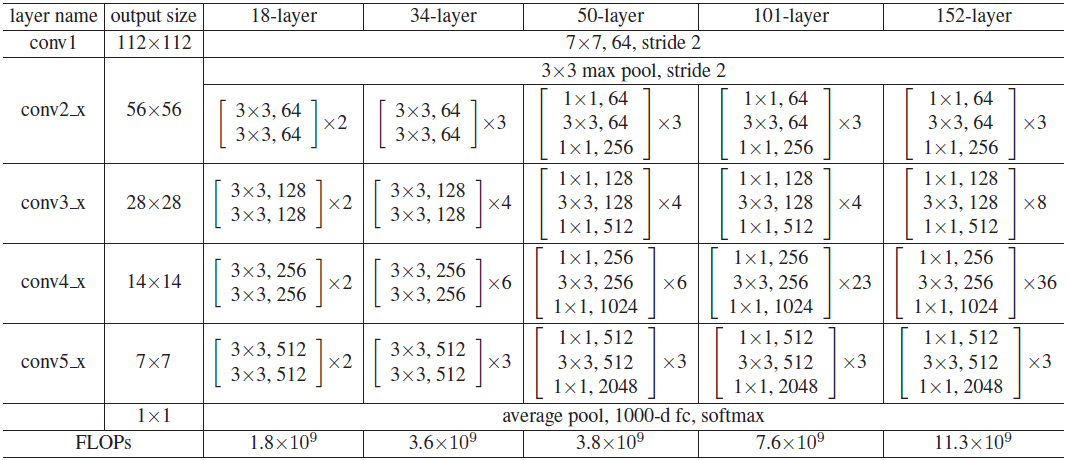
\includegraphics[width=\textwidth]{gambar/Arsitektur Residual Neural network untuk ImageNet.png}
%	\caption{Arsitektur Residual Neural Network untuk Implementasi ImageNet \parencite{ResNet}}
%	\label{fig:ArsResNet}
%\end{figure}


\begin{table}[hbtp]
    \centering
    \footnotesize
    \setlength{\tabcolsep}{2pt} % Adjust column separation
    \renewcommand{\arraystretch}{1.2} % Adjust row separation
    \begin{tabular}{|c|c|c|c|c|c|c|}
        \hline
        \textbf{Layer Name} & \textbf{Output Size} & \textbf{18-layer} & \textbf{34-layer} & \textbf{50-layer} & \textbf{101-layer} & \textbf{152-layer} \\
        \hline
        conv1 & 112$\times$112 & \multicolumn{5}{c|}{7$\times$7, 64, stride 2} \\
        \hline
        && \multicolumn{5}{c|}{3$\times$3 max pool, stride 2} \\
        \hline
        conv2\_x & 56$\times$56 & 
        \begin{tabular}{@{}c@{}}$\begin{bmatrix} 3 \times 3, 64 \\ 3 \times 3, 64 \end{bmatrix} \times 2$\end{tabular} & 
        \begin{tabular}{@{}c@{}}$\begin{bmatrix} 3 \times 3, 64 \\ 3 \times 3, 64 \end{bmatrix} \times 3$\end{tabular} & 
        \begin{tabular}{@{}c@{}}$\begin{bmatrix} 1 \times 1, 64 \\ 3 \times 3, 64 \\ 1 \times 1, 256 \end{bmatrix} \times 3$\end{tabular} & 
        \begin{tabular}{@{}c@{}}$\begin{bmatrix} 1 \times 1, 64 \\ 3 \times 3, 64 \\ 1 \times 1, 256 \end{bmatrix} \times 3$\end{tabular} & 
        \begin{tabular}{@{}c@{}}$\begin{bmatrix} 1 \times 1, 64 \\ 3 \times 3, 64 \\ 1 \times 1, 256 \end{bmatrix} \times 3$\end{tabular} \\
        \hline
        conv3\_x & 28$\times$28 & 
        \begin{tabular}{@{}c@{}}$\begin{bmatrix} 3 \times 3, 128 \\ 3 \times 3, 128 \end{bmatrix} \times 2$\end{tabular} & 
        \begin{tabular}{@{}c@{}}$\begin{bmatrix} 3 \times 3, 128 \\ 3 \times 3, 128 \end{bmatrix} \times 4$\end{tabular} & 
        \begin{tabular}{@{}c@{}}$\begin{bmatrix} 1 \times 1, 128 \\ 3 \times 3, 128 \\ 1 \times 1, 512 \end{bmatrix} \times 4$\end{tabular} & 
        \begin{tabular}{@{}c@{}}$\begin{bmatrix} 1 \times 1, 128 \\ 3 \times 3, 128 \\ 1 \times 1, 512 \end{bmatrix} \times 4$\end{tabular} & 
        \begin{tabular}{@{}c@{}}$\begin{bmatrix} 1 \times 1, 128 \\ 3 \times 3, 128 \\ 1 \times 1, 512 \end{bmatrix} \times 8$\end{tabular} \\
        \hline
        conv4\_x & 14$\times$14 & 
        \begin{tabular}{@{}c@{}}$\begin{bmatrix} 3 \times 3, 256 \\ 3 \times 3, 256 \end{bmatrix} \times 2$\end{tabular} & 
        \begin{tabular}{@{}c@{}}$\begin{bmatrix} 3 \times 3, 256 \\ 3 \times 3, 256 \end{bmatrix} \times 6$\end{tabular} & 
        \begin{tabular}{@{}c@{}}$\begin{bmatrix} 1 \times 1, 256 \\ 3 \times 3, 256 \\ 1 \times 1, 1024 \end{bmatrix} \times 6$\end{tabular} & 
        \begin{tabular}{@{}c@{}}$\begin{bmatrix} 1 \times 1, 256 \\ 3 \times 3, 256 \\ 1 \times 1, 1024 \end{bmatrix} \times 23$\end{tabular} & 
        \begin{tabular}{@{}c@{}}$\begin{bmatrix} 1 \times 1, 256 \\ 3 \times 3, 256 \\ 1 \times 1, 1024 \end{bmatrix} \times 36$\end{tabular} \\
        \hline
        conv5\_x & 7$\times$7 & 
        \begin{tabular}{@{}c@{}}$\begin{bmatrix} 3 \times 3, 512 \\ 3 \times 3, 512 \end{bmatrix} \times 2$\end{tabular} & 
        \begin{tabular}{@{}c@{}}$\begin{bmatrix} 3 \times 3, 512 \\ 3 \times 3, 512 \end{bmatrix} \times 3$\end{tabular} & 
        \begin{tabular}{@{}c@{}}$\begin{bmatrix} 1 \times 1, 512 \\ 3 \times 3, 512 \\ 1 \times 1, 2048 \end{bmatrix} \times 3$\end{tabular} & 
        \begin{tabular}{@{}c@{}}$\begin{bmatrix} 1 \times 1, 512 \\ 3 \times 3, 512 \\ 1 \times 1, 2048 \end{bmatrix} \times 3$\end{tabular} & 
        \begin{tabular}{@{}c@{}}$\begin{bmatrix} 1 \times 1, 512 \\ 3 \times 3, 512 \\ 1 \times 1, 2048 \end{bmatrix} \times 3$\end{tabular} \\
        \hline
        & 1$\times$1 & \multicolumn{5}{c|}{average pool, 1000-d fc, softmax} \\
        \hline
        & FLOPs & $1.8 \times 10^9$ & $3.6 \times 10^9$ & $3.8 \times 10^9$ & $7.6 \times 10^9$ & $11.3 \times 10^9$ \\
        \hline
    \end{tabular}
    \caption{Arsitektur Residual Neural Network untuk Implementasi ImageNet \parencite{ResNet}}
	\label{fig:ArsResNet}
\end{table}


\subsection{Confusion Matrix}
Ketika menilai efektivitas model klasifikasi, \emph{confusion matrix} merupakan komponen yang penting. Hal ini terutama berlaku ketika menganalisis gambar medis untuk tujuan seperti mendeteksi retinopati diabetik. Matriks ini menawarkan analisis menyeluruh tentang perbandingan prediksi model dan hasil aktual, sehingga memungkinkan untuk mengevaluasi keakuratan model dan menunjukkan area yang membutuhkan pengembangan.
Struktur confusion matrix adalah sebagai berikut:

\begin{longtable}{|c|c|c|}
    \caption{Confusion Matrix}
    \label{tb:confusion_matrix}                                  \\
    \hline
    & Predicted Negative & Predicted Positive \\
    \hline
    Actual Negative & True Negative (TN) & False Positive (FP) \\
    \hline
    Actual Positive & False Negative (FN) & True Positive (TP) \\
    \hline
\end{longtable}

\begin{itemize}
    \item \textbf{True Negative (TN)}: Jumlah instance negatif yang diprediksi dengan benar sebagai negatif.
    \item \textbf{False Positive (FP)}: Jumlah instance negatif yang diprediksi dengan salah sebagai positif.
    \item \textbf{False Negative (FN)}: Jumlah instance positif yang diprediksi dengan salah sebagai negatif.
    \item \textbf{True Positive (TP)}: Jumlah instance positif yang diprediksi dengan benar sebagai positif.
\end{itemize}

Confusion matrix memungkinkan kita untuk menghitung beberapa metrik penting:

\begin{itemize}
    \item \textbf{Accuracy}: $(TP + TN) / (TP + TN + FP + FN)$ - proporsi prediksi yang benar dari total.
    \item \textbf{Precision}: $TP / (TP + FP)$ - proporsi identifikasi positif yang benar.
    \item \textbf{Recall (Sensitivity)}: $TP / (TP + FN)$ - proporsi kasus positif aktual yang diidentifikasi dengan benar.
    \item \textbf{F1 Score}: $2 \times \frac{Precision \times Recall}{Precision + Recall}$ - rata-rata harmonik dari precision dan recall.
\end{itemize}

Metrik-metrik ini memberikan wawasan tentang berbagai aspek kinerja model. Misalnya, precision fokus pada akurasi prediksi positif, sementara recall menekankan kemampuan untuk mengidentifikasi semua kasus positif.

\subsection{Quadratic Weighted Kappa}

Quadratic Weighted Kappa (QWK) adalah ukuran statistik yang digunakan untuk mengevaluasi tingkat kesepakatan antara dua penguji atau pengklasifikasi, dengan mempertimbangkan kemungkinan kesepakatan secara kebetulan terjadi. Hal ini berguna dalam masalah klasifikasi multi-kelas, seperti penilaian keparahan retinopati diabetik, di mana kelas-kelas tersebut berurutan.

Nilai QWK berkisar dari -1 (ketidaksepakatan lengkap) hingga 1 (kesepakatan sempurna), dengan 0 menunjukkan kesepakatan yang setara dengan kebetulan.

QWK dapat dihitung dengan langkah-langkah sebagai berikut:

\begin{enumerate}
    \item \textbf{Buat Matriks Bobot \(W\)}:
    
    Setiap elemen \(W_{i,j}\) dari matriks didefinisikan sebagai \(\frac{(i - j)^2}{(N - 1)^2}\), di mana \(i\) dan \(j\) adalah indeks matriks, dan \(N\) adalah jumlah kelas.
    
    \item \textbf{Buat Confusion Matrix \(O\)}:
    
    Matriks ini berisi jumlah pengamatan dari kesepakatan antara dua penguji untuk setiap kelas.
    
    \item \textbf{Buat Expected Matriks \(E\)}:
     
    Matriks ini berisi jumlah pengamatan yang diharapkan dari kesepakatan antara dua penguji, yang dihitung berdasarkan hasil kali jumlah marginal dari matriks pengamatan \(O\).
    
    \item \textbf{Hitung QWK}:
    
    QWK kemudian didapatkan dengan:
    \[
    \kappa = 1 - \frac{\sum_{i,j} W_{i,j} O_{i,j}}{\sum_{i,j} W_{i,j} E_{i,j}}
    \]
\end{enumerate}

Dengan menggunakan QWK, kita dapat mengevaluasi kesepakatan antara kelas yang diprediksi dan aktual, dengan mempertimbangkan sifat kelas yang terurut, yang mana sangat relevan dalam diagnosis medis di mana tingkat keparahan suatu kondisi sering kali mengikuti urutan.

\subsection{Grad-CAM}
\label{sec:225}

Gradient-weighted Class Activation Mapping adalah alat yang membuat heatmap untuk menyorot area gambar yang menurut model deep learning paling penting untuk sebuah keputusan. Alat ini bekerja dengan menganalisis hubungan antara prediksi akhir dan fitur jaringan internal. Hal ini membantu men-debug model, mengidentifikasi bias, dan mengembangkan kepercayaan dalam keputusan AI.

\subsubsection{Prinsip Kerja Grad-CAM}

Grad-CAM bekerja dengan menggunakan gradien dari kelas yang diinginkan, yang mengalir kembali ke lapisan convolutional terakhir model untuk menghasilkan \emph{heatmap}. Berikut adalah langkah-langkah utama dalam Grad-CAM:

\begin{enumerate}
    \item \textbf{Mendapatkan Gradien:} Pertama, hitung gradien dari skor kelas target (misalnya, probabilitas kelas tertentu) terhadap fitur map dari lapisan convolutional terakhir.
    \item \textbf{Menghitung Bobot:} Rata-rata gradien ini di seluruh dimensi spasial untuk mendapatkan bobot penting, yang menunjukkan seberapa penting fitur tertentu untuk kelas yang diinginkan.
    \item \textbf{Menghasilkan \emph{heatmap}:} Buat \emph{heatmap} sebagai kombinasi linier dari fitur map dan bobot yang diperoleh. \emph{heatmap} ini menunjukkan area pada gambar asli yang memiliki pengaruh terbesar terhadap prediksi model.
\end{enumerate}

Secara matematis, \emph{heatmap} \(L_{\text{Grad-CAM}}^c\) untuk kelas \(c\) dihitung sebagai berikut:

\[
L_{\text{Grad-CAM}}^c = \text{ReLU}\left(\sum_k \alpha_k^c A^k\right)
\]

Di mana:

\begin{itemize}
    \item \(A^k\) adalah peta fitur dari lapisan convolutional terakhir.
    \item \(\alpha_k^c\) adalah bobot penting yang dihitung sebagai rata-rata gradien dari skor kelas \(c\) terhadap \(A^k\).
    \item \(\text{ReLU}\) adalah fungsi aktivasi Rectified Linear Unit yang memastikan hanya nilai positif yang dipertimbangkan, menghilangkan pengaruh negatif.
\end{itemize}

\subsubsection{Kelebihan Grad-CAM}

Grad-CAM memiliki beberapa kelebihan yang membuatnya sangat berguna dalam analisis dan interpretasi model pembelajaran mendalam:

\begin{itemize}
    \item \textbf{Generalisasi:} Grad-CAM dapat digunakan dengan berbagai arsitektur CNN tanpa memerlukan modifikasi khusus pada model.
    \item \textbf{Keterlihatan:} \emph{heatmap} yang dihasilkan memberikan wawasan visual yang intuitif tentang area gambar yang paling berpengaruh pada keputusan model, membantu dalam diagnosis dan debugging model.
    \item \textbf{Fleksibilitas:} Grad-CAM dapat diterapkan pada berbagai tugas klasifikasi, termasuk deteksi objek dan segmentasi, dengan memberikan interpretasi yang lebih baik tentang bagaimana model memandang input \parencite{selvaraju2017grad}.
\end{itemize}

\subsubsection{Aplikasi Grad-CAM}

Grad-CAM telah digunakan dalam berbagai aplikasi di bidang pengolahan citra dan visi komputer, termasuk:

\begin{itemize}
    \item \textbf{Deteksi Penyakit Medis:} Grad-CAM membantu dalam memahami prediksi model untuk deteksi penyakit dari citra medis, seperti mammografi, radiografi, dan retinografi.
    \item \textbf{Sistem Pengawasan:} Dalam sistem pengawasan otomatis, Grad-CAM membantu dalam memahami area yang diprioritaskan oleh model dalam mendeteksi aktivitas mencurigakan.
    \item \textbf{Kendaraan Otonom:} Pada kendaraan otonom, Grad-CAM membantu dalam menganalisis bagaimana model memutuskan tindakan berdasarkan citra dari sensor kamera \parencite{selvaraju2017grad}.
\end{itemize}

Grad-CAM merupakan alat yang cukup kuat dalam interpretasi model \emph{deepl learning}, memberikan kepercayaan lebih dalam penggunaan model ini pada aplikasi di dunia nyata.

